% fig03_pipeline.tex — TikZ 10-stage D-T fuel flow diagram for §Full Pipeline.
% Compiled by the paper Makefile via `make figures` (pdflatex on the snippet).
% Tier-color-coded: green = sim-PASS (closed in this funnel), orange = wet-lab /
% out-of-scope (NOT closed). The tier word is inside the node so the diagram is
% independently readable without cross-referencing the §Full Pipeline table.
%
% Manual single-shot compile (debug):
%   pdflatex -interaction=nonstopmode -halt-on-error fig03_pipeline.tex
\documentclass[tikz,border=4pt]{standalone}
\usetikzlibrary{positioning,arrows.meta,shapes.geometric}
\begin{document}
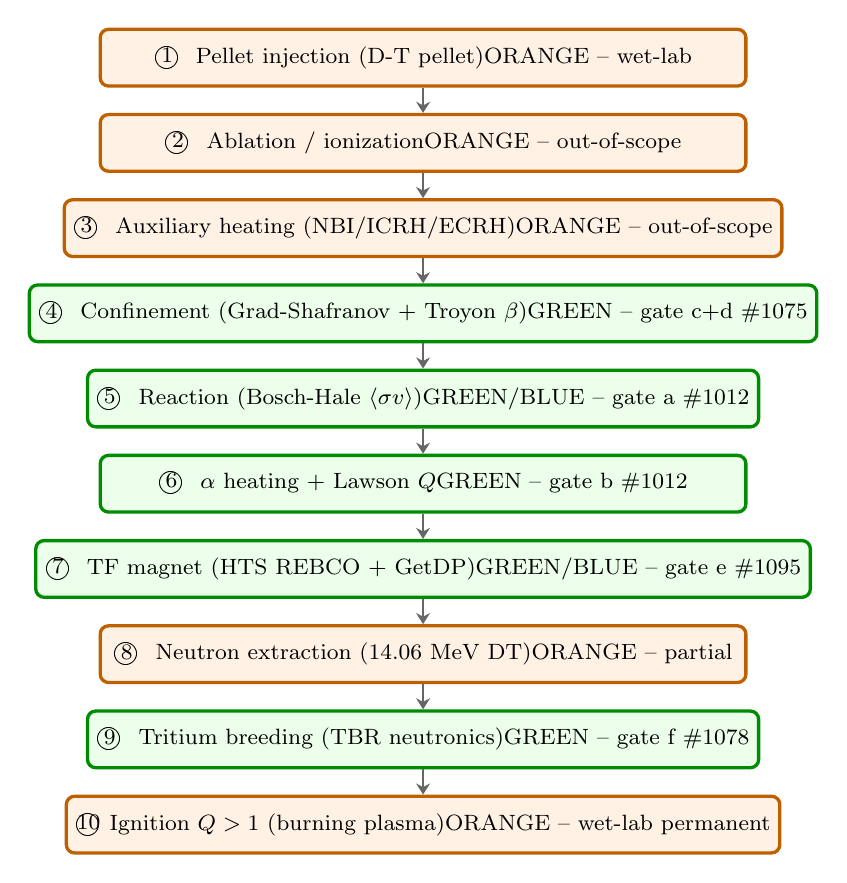
\begin{tikzpicture}[
  font=\footnotesize,
  closed/.style = {
    rectangle, rounded corners=3pt, draw=green!55!black, very thick,
    minimum width=8.2cm, minimum height=0.72cm, align=left,
    fill=green!8,
  },
  wet/.style = {
    rectangle, rounded corners=3pt, draw=orange!75!black, very thick,
    minimum width=8.2cm, minimum height=0.72cm, align=left,
    fill=orange!10,
  },
  arrow/.style = {-{Stealth[length=4pt,width=5pt]}, thick, draw=black!60},
  node distance=0.32cm,
]
  \node[wet]                  (s1)  {\textcircled{1}\ \ Pellet injection (D-T pellet)\hfill ORANGE -- wet-lab};
  \node[wet,    below=of s1]  (s2)  {\textcircled{2}\ \ Ablation / ionization\hfill ORANGE -- out-of-scope};
  \node[wet,    below=of s2]  (s3)  {\textcircled{3}\ \ Auxiliary heating (NBI/ICRH/ECRH)\hfill ORANGE -- out-of-scope};
  \node[closed, below=of s3]  (s4)  {\textcircled{4}\ \ Confinement (Grad-Shafranov + Troyon $\beta$)\hfill GREEN -- gate c+d \#1075};
  \node[closed, below=of s4]  (s5)  {\textcircled{5}\ \ Reaction (Bosch-Hale $\langle\sigma v\rangle$)\hfill GREEN/BLUE -- gate a \#1012};
  \node[closed, below=of s5]  (s6)  {\textcircled{6}\ \ $\alpha$ heating + Lawson $Q$\hfill GREEN -- gate b \#1012};
  \node[closed, below=of s6]  (s7)  {\textcircled{7}\ \ TF magnet (HTS REBCO + GetDP)\hfill GREEN/BLUE -- gate e \#1095};
  \node[wet,    below=of s7]  (s8)  {\textcircled{8}\ \ Neutron extraction (14.06 MeV DT)\hfill ORANGE -- partial};
  \node[closed, below=of s8]  (s9)  {\textcircled{9}\ \ Tritium breeding (TBR neutronics)\hfill GREEN -- gate f \#1078};
  \node[wet,    below=of s9]  (s10) {\textcircled{10}\ Ignition $Q>1$ (burning plasma)\hfill ORANGE -- wet-lab permanent};

  \draw[arrow] (s1)  -- (s2);
  \draw[arrow] (s2)  -- (s3);
  \draw[arrow] (s3)  -- (s4);
  \draw[arrow] (s4)  -- (s5);
  \draw[arrow] (s5)  -- (s6);
  \draw[arrow] (s6)  -- (s7);
  \draw[arrow] (s7)  -- (s8);
  \draw[arrow] (s8)  -- (s9);
  \draw[arrow] (s9)  -- (s10);
\end{tikzpicture}
\end{document}
